\documentclass[tikz]{standalone}
\usepackage{fontspec}
\renewcommand*{\familydefault}{\sfdefault}
\usepackage{standalone}
\usetikzlibrary{arrows.meta, decorations.pathreplacing, shapes.geometric}
%\usetikzlibrary{positioning,fit,shapes.geometric,fadings,bayesnet}

\begin{document}

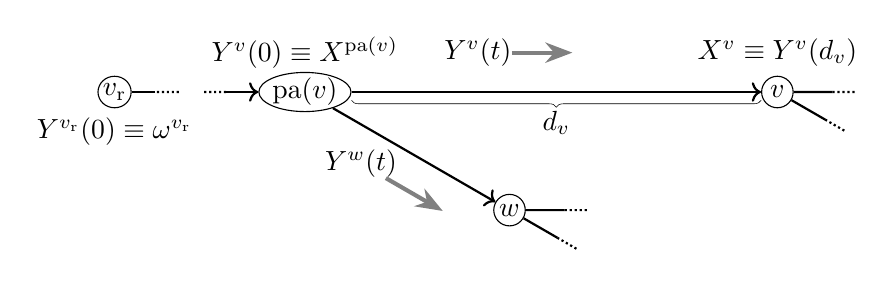
\begin{tikzpicture}[
%label position=0,
radius=2 pt,
treenode/.style={
ellipse,
draw,
minimum size=0.4 cm,
inner sep=0 pt,
}
]

% tree nodes
\node [treenode] at (0,0) (pa)
{\(\mathrm{pa}(v)\)};
\node [treenode] at (0:6 cm) (v)  {\(v\)};
\node [treenode] at (-30:3 cm) (w)  {\(w\)};

\draw [thick, ->] (pa) -- node[midway,] {}(w);
\draw [thick, ->] (pa) -- (v);
\draw[very thin, decorate, decoration={brace, mirror, raise=3 pt}] (pa) --
node[midway, label=below:\(d_v\)]{} (v);

% truncated edges
\draw[thick, solid]
(v) -- +(0:0.7 cm) coordinate(v1)
(v) -- +(-30:0.7 cm) coordinate(v2)
(w) -- +(0:0.7 cm) coordinate(w1)
(w) -- +(-30:0.7 cm) coordinate(w2)
;
\draw [thick, solid, ->] (180:1.0 cm) coordinate(pa1) -- (pa);
\draw[thick,densely dotted]
(v1) -- +(0:0.3 cm)
(v2) -- +(-30:0.3 cm)
(w1) -- +(0:0.3 cm)
(w2) -- +(-30:0.3 cm)
(pa1) -- ++(180:0.3 cm)
++(180:0.3 cm) -- ++(180:0.3 cm) coordinate (root1)
;
\draw[thick, solid] (root1) -- +(180:0.3 cm) node[treenode, anchor=east,thin]
(root) {\(v_\mathrm{r}\)};

% substitution process on branch b_v
\path
(pa) +(90:0.5 cm) node (Y0) {\(Y^v(0)\equiv X^{\mathrm{pa}(v)}\)}
(v) +(90:0.5 cm) node (Ydv) {\(X^v\equiv Y^v(d_v)\)}
(root) +(-90:0.5 cm) node (Yroot0) {\(Y^{v_\mathrm{r}}(0)\equiv \omega^{v_\mathrm{r}}\)}
;
\path[] (Y0) -- node[near start, inner sep=0 pt] (Yt) {\(Y^v(t)\)} (Ydv);
\draw[gray, line width=1.5 pt, arrows={-Stealth}] (Yt) -- +(0:1.2 cm);

% substitution process on branch b_w
\path
(pa) +(-90:0.5 cm) node (Yw0) {}
(w) +(-90:0.5 cm) node (Ywdv) {}
;
\path[] (Yw0) -- node[near start, inner sep=0 pt] (Ywt) {\(Y^w(t)\)} (Ywdv);
\draw[gray, line width=1.5 pt, arrows={-Stealth}] (Ywt) -- +(-30:1.2 cm);

\end{tikzpicture}
\end{document}
